%%%%%%%%%%%%%%%%%%%%%%%%%%%%%%%%%%%%%%%%%%%%%%%%%%%%%%%%%%%%%%%%%%%%%%%%
%  
%  Use of biom.cls and the template to typeset an already published
%  Biometrics article:
%
%  Verbeke, G. and Molenberghs, G. (2003).  The use of score tests for
%     inference on variance components.  Biometrics 59, 254-262.
%
%  The format of the two-column typeset version produced by biom.cls
%  differs a bit from that published in 2003 owing to some differences
%  in formatting parameters.  
%
%  The LaTeX source kindly provided by these authors has been ``dropped''
%  into the template file with little modification.
%
%%%%%%%%%%%%%%%%%%%%%%%%%%%%%%%%%%%%%%%%%%%%%%%%%%%%%%%%%%%%%%%%%%%%%%%%

\documentclass[useAMS,usenatbib,referee]{biom}

\newcommand{\Yi}{\bm{Y_i}}
\newcommand{\Yiobs}{\bm{Y_i}^{\! o}}
\newcommand{\yiobs}{\bm{y_i}^{\! o}}
\newcommand{\h}{\mbox{\boldmath $h$}}
\newcommand{\etal}{et al.\ }
%\newcommand{\bm}[1]{\mbox{\boldmath $#1$}}
\newcommand{\subN}{\mbox{\tiny N}}
\newcommand{\subX}{\mbox{\tiny X}}
\newcommand{\subML}{\mbox{\tiny ML}}
\newcommand{\subREML}{\mbox{\tiny REML}}
\newcommand{\subZ}{\mbox{\tiny Z}}
\newcommand{\subO}{\mbox{\tiny $0$}}
\newcommand{\subeen}{\mbox{\tiny $1$}}
\newcommand{\subtwee}{\mbox{\tiny $2$}}
\newcommand{\subOLS}{\mbox{\tiny OLS}}
\newcommand{\subA}{\mbox{\tiny A}}
\newcommand{\subB}{\mbox{\tiny B}}
\newcommand{\subC}{\mbox{\tiny C}}
\newcommand{\subI}{\mbox{\tiny I}}
\newcommand{\subK}{\mbox{\tiny K}}
\newcommand{\subR}{\mbox{\tiny R}}
\newcommand{\subF}{\mbox{\tiny F}}
\newcommand{\vc}{\mbox{vec}}
\newcommand{\subM}{\mbox{\tiny M}}
\newcommand{\subH}{\mbox{\tiny H}}
\newcommand{\subAIC}{\mbox{\tiny AIC}}
\newcommand{\subSBC}{\mbox{\tiny SBC}}
\newcommand{\subQ}{\mbox{\tiny Q}}
\newcommand{\bhoed}{\widehat{\bm{b_i}}}
\newcommand{\bbhoed}{\widehat{\bm{B_i}}}
\newcommand{\ahoed}{\widehat{\bm\alpha}}
\newcommand{\thoed}{\widehat{\bm\theta}}
\newcommand{\whoed}{\widehat{W_i}}
\newcommand{\psihoed}{\widehat{\bm\psi}_{\subN}}
\newcommand{\epsi}{\bm{\varepsilon_i}}

\newcommand{\epsei}{\bm{\varepsilon_{\subeen i}}}
\newcommand{\epsti}{\bm{\varepsilon_{\subtwee i}}}

\newcommand{\ei}{\bm{e_i}}
\newcommand{\yi}{\bm{y_i}}
\newcommand{\ri}{\bm{r_i}}
\newcommand{\reri}{\bm{\Re_i}}
\newcommand{\bi}{\bm{b_i}}
\newcommand{\calr}{\mbox{$\bm{{\cal R}}$}}
\newcommand{\calx}{\mbox{${\cal X}$}}
\newcommand{\calp}{\mbox{${\cal P}$}}
\newcommand{\calz}{\mbox{${\cal Z}$}}
\newcommand{\caln}{\mbox{${\cal N}$}}
\newcommand{\caly}{\mbox{${\cal Y}$}}
\newcommand{\cala}{\mbox{${\cal A}$}}
\newcommand{\calage}{\mbox{${\cal A}ge$}}
\newcommand{\vinv}{\mbox{$V_i^{-1}$}}
\newcommand{\vinvtwee}{\mbox{$V_i^{-1/2}$}}
\newcommand{\zk}{\mbox{$Z_i^{(k)}$}}
\newcommand{\zl}{\mbox{$Z_i^{(l)}$}}
\newcommand{\ak}{\mbox{$A_i^{(k)}$}}
\newcommand{\aj}{\mbox{$A_i^{(j)}$}}
\newcommand{\zp}{\mbox{$Z_i^{(p)}$}}
\newcommand{\zq}{\mbox{$Z_i^{(q)}$}}
\newcommand{\tr}{\mbox{tr}}
\newcommand{\anmin}{\mbox{$\ddot{L}^{-1}$}}

\newcommand{\xieen}{X_i^{(1)}}
\newcommand{\xitwee}{X_i^{(2)}}
\newcommand{\betaeen}{\bm\beta^{(1)}}
\newcommand{\betatwee}{\bm\beta^{(2)}}
\newcommand{\zieen}{Z_i^{(1)}}
\newcommand{\zitwee}{Z_i^{(2)}}
\newcommand{\bieen}{b_i^{(1)}}
\newcommand{\bitwee}{\bm{b_i}^{(2)}}
\newcommand{\een}{\bm{1_{n_i}}}
\newcommand{\yigem}{\overline{\bm{y}}_i}

\newcommand{\xeen}{X^{(1)}}
\newcommand{\xtwee}{X^{(2)}}
\newcommand{\zeen}{Z^{(1)}}
\newcommand{\ztwee}{Z^{(2)}}
\newcommand{\been}{\bm{b}^{(1)}}
\newcommand{\btwee}{\bm{b}^{(2)}}
\newcommand{\btweenul}{\bm{b_0^{(2)}}}
\newcommand{\y}{\bm{y}}
\newcommand{\e}{\bm{e}}
\newcommand{\boldb}{\bm{b}}


\newcommand{\BSig}{\mbox{\unboldmath{$\Sigma$}}}                 
 \newcommand{\comb}[2]{\left(\begin{array}{c}{{#1}}\\{{#2}}\end{array}\right)}
 \newcommand{\matt}[4]{\left(\begin{array}{cc}{{#1}}&{{#2}}\\{{#3}}&{{#4}}    
            \end{array}\right)}                    

 \newcommand{\br}{\mbox{\boldmath{$r$}}}                     
 \newcommand{\bea}{\mbox{\boldmath{$e_1$}}}                   
 \newcommand{\beb}{\mbox{\boldmath{$e_2$}}}                   
 \newcommand{\bej}{\mbox{\boldmath{$e_j$}}}                   
 \newcommand{\rP}{P}                           
 \newcommand{\rE}{E}                           
 \newcommand{\Bmur}{\Bmu^{(r)}}
 \newcommand{\Bmud}{\Bmu{(d)}}
 \newcommand{\Bmut}{\Bmu{(d)}}
\newcommand{\BSigr}{\Sigma^{(r)}}
\newcommand{\BSigd}{\Sigma{(d)}}
\newcommand{\BSigt}{\Sigma{(d)}}
\newcommand{\Bmu}{\mbf{\mu}}
\newcommand{\rN}{\mbox{N}}
\newcommand{\mat}[2]{\mbox{$\left(\begin{array}{#1}#2\end{array}\right)$}}
\newcommand{\mbf}[1]{\mbox{\boldmath$#1$}}

 \newcommand{\saa}{\sigma_{11}}                         
 \newcommand{\sab}{\sigma_{12}}                         
 \newcommand{\sbb}{\sigma_{22}}                       
 \newcommand{\yprev}{Y_{_{\mbox{\tiny pr}}}}
 \newcommand{\ycurr}{Y_{_{\mbox{\tiny c}}}}
 \newcommand{\Cov}{\mbox{Cov}}
 \newcommand{\bitem}{\begin{itemize}}
 \newcommand{\eitem}{\end{itemize}}
 \newcommand{\vet}[1]{\mbox{\boldmath $#1$}}
 \newcommand{\vetje}[1]{\mbox{\boldmath $\scriptstyle #1$}}
 \newcommand{\pmin}{\phantom{-}}
 \newcommand{\pvert}{\phantom{|}}
 \newcommand{\recht}[1]{\mbox{#1}}
 \newcommand{\hoogte}{\rule{0pt}{\baselineskip}}
 \newcommand{\hoogteke}[1]{\rule{0pt}{#1}}
 \newcommand{\Ran}{\mbox{Ran}}
 \newcommand{\sst}{\scriptstyle}
 \newcommand{\ds}{\displaystyle}
 \newcommand{\CD}{\protect\mbox{\rm CD}}
 \newcommand{\p}{\mbox{\rm p}}
 \newcommand{\pp}{\mbox{\rm P}}
 \newcommand{\fakestde}{\mbox{$\phantom{(0.00)}$}}
 
 \newcommand{\x}{\mbox{\boldmath $x$}}
 \newcommand{\alp}{\mbox{\boldmath $\alpha$}}
 \newcommand{\bet}{\mbox{\boldmath $\beta$}}
 \newcommand{\betah}{\mbox{$\widehat{\beta}$}}
 \newcommand{\epsilonh}{\mbox{$\widehat{\epsilon}$}}
 \newcommand{\beps}{\mbox{\boldmath $\varepsilon$}}
 \newcommand{\betaw}{\mbox{$\tilde{\bet}_W$}}
 \newcommand{\beth}{\mbox{$\widehat{\bet}$}}
 \newcommand{\bepsh}{\mbox{$\widehat{\beps}$}}
 \newcommand{\gam}{\mbox{\boldmath $\gamma$}}
 \newcommand{\vpsi}{\vet{\psi}}
 \newcommand{\vt}{\mbox{$\vet{\theta}$}}
 \newcommand{\bmu}{\mbox{\boldmath $\mu$}}
 \newcommand{\bnu}{\mbox{\boldmath $\nu$}}
 \newcommand{\bdelta}{\mbox{\boldmath $\delta$}}
 \newcommand{\btau}{\mbox{\boldmath $\tau$}}
 \newcommand{\bLambda}{\mbox{\boldmath $\Lambda$}}
 \newcommand{\blambda}{\mbox{\boldmath $\lambda$}}
 \newcommand{\bflambda}{\mbox{\boldmath $\lambda$}}
 \newcommand{\bSigma}{\mbox{\boldmath $\Sigma$}}
 \newcommand{\bOmega}{\mbox{\boldmath $\Omega$}}
 \newcommand{\bPsi}{\mbox{\boldmath $\Psi$}}
\newcommand{\bpsi}{\mbox{\boldmath $\psi$}}
 \newcommand{\bsigma}{\mbox{\boldmath $\sigma$}}
 \newcommand{\bSigmah}{\mbox{$\widehat{\bSigma}$}}
 \newcommand{\brho}{\mbox{\boldmath $\rho$}}
 \newcommand{\boeta}{\mbox{\boldmath $\eta$}}
 \newcommand{\nul}{\mbox{\bfseries 0}}
 \newcommand{\rechts}{\phantom{.}\hfill}
 \newcommand{\W}{\mbox{\boldmath $W$}}
 \newcommand{\BA}{\mbox{\boldmath $A$}}
 \newcommand{\ba}{\mbox{\boldmath $a$}}
 \newcommand{\bd}{\mbox{\boldmath $d$}}
 \newcommand{\bg}{\mbox{\boldmath $g$}}
 %\newcommand{\bh}{\mbox{\boldmath $h$}}
 \newcommand{\bw}{\mbox{\boldmath $w$}}
 \newcommand{\BB}{\mbox{\boldmath $B$}}
 \newcommand{\BM}{\mbox{\boldmath $M$}}
 \newcommand{\BN}{\mbox{\boldmath $N$}}
 \newcommand{\BC}{\mbox{\boldmath $C$}}
 \newcommand{\BD}{\mbox{\boldmath $D$}}
 \newcommand{\BE}{\mbox{\boldmath $E$}}
 \newcommand{\BH}{\mbox{\boldmath $H$}}
 \newcommand{\bh}{\mbox{\boldmath $h$}}

 \newcommand{\BK}{\mbox{\boldmath $K$}}
 \newcommand{\BG}{\mbox{\boldmath $G$}}
 \newcommand{\BR}{\mbox{\boldmath $R$}}
 \newcommand{\BQ}{\mbox{\boldmath $Q$}}
 \newcommand{\BS}{\mbox{\boldmath $S$}}
 \newcommand{\bs}{\mbox{\boldmath $s$}}
 \newcommand{\BV}{\mbox{\boldmath $V$}}
 \newcommand{\BW}{\mbox{\boldmath $W$}}
 \newcommand{\BY}{\mbox{\boldmath $Y$}}
 \newcommand{\BX}{\mbox{\boldmath $X$}}
 \newcommand{\BP}{\mbox{\boldmath $P$}}
 \newcommand{\X}{\mbox{\boldmath $X$}}
 \newcommand{\BU}{\mbox{\boldmath $U$}}
 \newcommand{\BJ}{\mbox{\boldmath $J$}}
 \newcommand{\BI}{\mbox{\boldmath $I$}}
 \newcommand{\bx}{\mbox{\boldmath $x$}}
%\newcommand{\bq}{\mbox{\boldmath $q$}}
 \newcommand{\by}{\mbox{\boldmath $y$}}
  \newcommand{\byo}{\mbox{\boldmath{$\by_o$}}} 
 \newcommand{\bym}{\mbox{\boldmath{$\by_m$}}}
  \newcommand{\bt}{\mbox{\boldmath $t$}}
 \newcommand{\bu}{\mbox{\boldmath $u$}}
 \newcommand{\byh}{\mbox{$\widehat{\by}$}}
 \newcommand{\BYH}{\mbox{$\widehat{\BY}$}}
 \newcommand{\be}{\mbox{\boldmath $e$}}
 \newcommand{\bv}{\mbox{\boldmath $v$}}
 \newcommand{\BZ}{\mbox{\boldmath $Z$}}
 \newcommand{\bz}{\mbox{\boldmath $z$}}
 \newcommand{\xbarj}[1]{\mbox{$\overline{x}_{#1}$}}
 \newcommand{\xbar}{\mbox{$\overline{\bx}$}}
 \newcommand{\xb}{\mbox{$\overline{x}$}}
 \newcommand{\yb}{\mbox{$\overline{y}$}}
 \newcommand{\Xbar}{\mbox{$\overline{\BX}$}}
 \newcommand{\Ybar}{\mbox{$\overline{\BY}$}}
 \newcommand{\Zbar}{\mbox{$\overline{\BZ}$}}
 \newcommand{\Dbar}{\mbox{$\overline{\BD}$}}
 \newcommand{\dbar}{\mbox{$\overline{\bd}$}}
 \newcommand{\ybar}{\mbox{$\overline{\by}$}}
 \newcommand{\Spooled}{\mbox{$\BS_{\mbox{\scriptsize pooled}}$}}
 \newcommand{\Spooledinv}{\mbox{$\BS_{\mbox{\scriptsize pooled}}^{-1}$}}
 
 \newcommand{\bxi}{\mbox{$\bx_i$}}
 \newcommand{\byi}{\mbox{$\by_i$}}
 \newcommand{\BXi}{\mbox{$\BX_i$}}
 \newcommand{\BZi}{\mbox{$\BZ_i$}}
 \newcommand{\BVi}{\mbox{$\BV_{i}$}}
 \newcommand{\BVih}{\mbox{$\widehat{\BVi}$}}
 \newcommand{\BWi}{\mbox{$\BW_{i}$}}
 \newcommand{\BWih}{\mbox{$\widehat{\BWi}$}}
 \newcommand{\BDi}{\mbox{$\BD_i$}}
 \newcommand{\BDih}{\mbox{$\widehat{\BDi}$}}
 \newcommand{\BRi}{\mbox{$\BR_i$}}
 \newcommand{\BZERO}{\mbox{\boldmath $0$}}
 
 \newcommand{\muij}{\mbox{$\mu_{ij}$}}
 \newcommand{\bmui}{\mbox{$\bmu_i$}}
 \newcommand{\bmuh}{\mbox{$\widehat{\bmu}$}}
 \newcommand{\bmuih}{\mbox{$\bmuh_i$}}
 \newcommand{\bb}{\mbox{\boldmath $b$}}
 \newcommand{\bc}{\mbox{\boldmath $c$}}
 \newcommand{\bbone}{\mbox{\boldmath $\beta_1$}}
 \newcommand{\bbh}{\mbox{$\widehat{\bb}$}}
 \newcommand{\bbhone}{\mbox{$\widehat{\bb}_1$}}
 \newcommand{\etaij}{\mbox{$\eta_{ij}$}}
 \newcommand{\boetai}{\mbox{$\boeta_i$}}
 \newcommand{\bl}{\mbox{\boldmath $\ell$}}
 \newcommand{\BL}{\mbox{\boldmath $L$}}
 \newcommand{\BHh}{\mbox{$\widehat{\BH}$}}
 \newcommand{\BXk}{\mbox{$\BX_k$}}
 \newcommand{\BZk}{\mbox{$\BZ_k$}}
 \newcommand{\BVk}{\mbox{$\BV_{k}$}}
 \newcommand{\BVkh}{\mbox{$\widehat{\BVk}$}}
 \newcommand{\BWk}{\mbox{$\BW_{k}$}}
 \newcommand{\BWkh}{\mbox{$\widehat{\BWk}$}}
 \newcommand{\BDk}{\mbox{$\BD_k$}}
 \newcommand{\BDkh}{\mbox{$\widehat{\BDk}$}}
 \newcommand{\BRk}{\mbox{$\BR_k$}}
 \newcommand{\byk}{\mbox{\boldmath $y_{k}$}}
 \newcommand{\bzk}{\mbox{\boldmath $z_{k}$}}
 \newcommand{\mukj}{\mbox{$\mu_{kj}$}}
 \newcommand{\bmuk}{\mbox{$\bmu_k$}}
 \newcommand{\bmukh}{\mbox{$\bmuh_k$}}
 \newcommand{\etakj}{\mbox{$\eta_{kj}$}}
 \newcommand{\boetak}{\mbox{$\boeta_k$}}
 \newcommand{\tn}{\mbox{$\widehat{\vt}_K$}}
 \newcommand{\ttilde}{\mbox{$\tilde{\vt}_K$}}
 \newcommand{\tast}{\mbox{$\vt_{\ast}$}}
 \newcommand{\gtn}{\mbox{$\tilde{\vet{\gamma}}_K$}}
 \newcommand{\pj}{p_{\vet{j}}}
 \newcommand{\yj}{y_{\vet{j}}}
 
 \newcommand{\ymis}{\mbox{$Y_{\mbox{\small m}}$}}
 \newcommand{\yobs}{\mbox{$Y_{\mbox{\small o}}$}}
 \newcommand{\zmis}{\mbox{$\BZ_{\mbox{\small m}}$}}
 \newcommand{\zobs}{\mbox{$\BZ_{\mbox{\small o}}$}}
 
 \newcommand{\SStr}{\mbox{$SS_{\mbox{tr}}$}}
 \newcommand{\SSres}{\mbox{$SS_{\mbox{res}}$}}
 
 \newcommand{\suml}{\sum_{\ell=1}^g}
 \newcommand{\sumk}{\sum_{k=1}^b}
 \newcommand{\sumi}{\sum_{i=1}^{n_\ell}}
 
 \newcommand{\bfY}{{\bfseries Y}}
 \newcommand{\bfy}{{\bfseries y}}
 \newcommand{\bfsigma}{\mbox{\boldmath $\sigma$}}
 \newcommand{\bfpsi}{\mbox{\boldmath $\psi$}}
 \newcommand{\bfpi}{\mbox{\boldmath $\pi$}}
 \newcommand{\bfgamma}{\mbox{\boldmath $\gamma$}}
 \newcommand{\bfSigma}{\mbox{\boldmath $\Sigma$}}
 \newcommand{\bftheta}{\mbox{\boldmath $\theta$}}
 \newcommand{\bfomega}{\mbox{\boldmath $\omega$}}
 \newcommand{\bfmu}{\mbox{\boldmath $\mu$}}
 \newcommand{\bfr}{ {\bfseries r} }
 \newcommand{\bfzero}{{\bfseries 0}}
 \newcommand{\hatF}{{ \widehat {F} }}
 \newcommand{\hf}{{ \widehat {f} }}
 \newcommand{\hatW}{{ \widehat {W} }}
 \newcommand{\hbff}{{ \widehat {\bfseries f} }}
 \newcommand{\hatB}{{ \widehat {B} }}
 \newcommand{\hmu}{{ \widehat {\mu} }}
 
 \newcommand{\bhat}{\widehat{\mbox{\boldmath$\beta$}}}
 \newcommand{\bbar}{\bar{\mbox{\boldmath$\beta$}}}
 \newcommand{\that}{\widehat{\mbox{\boldmath$\theta$}}}
 \newcommand{\ghat}{\widehat{\mbox{\boldmath$\gamma$}}}
 \newcommand{\ahat}{\widehat{\mbox{\boldmath$\alpha$}}}
 \newcommand{\htheta}{\widehat{\theta}}
 \newcommand{\ttheta}{\tilde{\theta}}
 \newcommand{\hgamma}{\widehat{\gamma}}
 \newcommand{\Var}{{\rm var}}
 \newcommand{\pr}{{\rm pr}}
 \newcommand{\obs}{{\rm obs}}
 \newcommand{\mis}{{\rm mis}}
 \newcommand{\invoeg}[2]
 {
 \begin{center}
 \framebox[16cm]{\hoogteke{#1} #2}
 \end{center}
 }
 \newcommand{\I}{\mbox{\boldmath $I$}}
 \newcommand{\Wi}{\mbox{\boldmath $W_{\mbox{\boldmath$i$}}$}}
 \newcommand{\V}{\mbox{\boldmath $V$}}
 \newcommand{\U}{\mbox{\boldmath $U$}}
 \newcommand{\R}{\mbox{\boldmath $R$}}
 \newcommand{\Y}{\mbox{\boldmath $Y$}}
 \newcommand{\D}{\mbox{\boldmath $D$}}
 \newcommand{\B}{\mbox{\boldmath $B$}}
 \newcommand{\Z}{\mbox{\boldmath $Z$}}
 \newcommand{\bfeta}{ {\mbox{\boldmath $\eta$}} }
 \newcommand{\bfnu}{ {\mbox{\boldmath $\nu$}} }
 \newcommand{\bfU}{ {\bfseries U} }
 \newcommand{\bfW}{ {\bfseries W} }
 \newcommand{\bfP}{ {\bfseries P} }
 \newcommand{\bfH}{ {\bfseries H} }
 \newcommand{\z}{\mbox{\boldmath $z$}}
 \newcommand{\zi}{\mbox{\boldmath $z_{\mbox{\boldmath$i$}}$}}
 \newcommand{\bfbeta}{\mbox{\boldmath $\beta$}}
 \newcommand{\vSigma}{\mbox{\boldmath $\Sigma$}}
 \newcommand{\vbeta}{\mbox{\boldmath $\beta$}}
 \newcommand{\valpha}{\mbox{\boldmath $\alpha$}}
 \newcommand{\vgamma}{\mbox{\boldmath $\gamma$}}
 \newcommand{\si}{\mbox{\boldmath $s_{\mbox{\boldmath$i$}}$}}
 \newcommand{\vmu}{\mbox{\boldmath $\mu$}}
 \newcommand{\vmui}{\mbox{\boldmath $\mu_{\mbox{\boldmath$i$}}$}}
 \newcommand{\vtau}{\mbox{\boldmath $\tau$}}
 \newcommand{\vTheta}{\mbox{\boldmath $\Theta$}}
 \newcommand{\Xie}{\mbox{\boldmath $X_{\mbox{\boldmath$i$}}$}}
 \newcommand{\zbar}{\mbox{\boldmath $\overline{z}$}}
 \newcommand{\Corr}{  {\rm Corr}  }




%\def\bSig\mathbf{\Sigma}
%\newcommand{\VS}{V\&S}
%\newcommand{\tr}{\mbox{tr}}


%  The rotating package allows you to have tables displayed in landscape
%  mode.  The rotating package is NOT included in this distribution, but
%  can be obtained from the CTAN archive.  USE OF LANDSCAPE TABLES IS
%  STRONGLY DISCOURAGED -- create landscape tables only as a last resort if
%  you see no other way to display the information.  If you do do this,
%  then you need the following command.

\usepackage[figuresright]{rotating}

%%%%%%%%%%%%%%%%%%%%%%%%%%%%%%%%%%%%%%%%%%%%%%%%%%%%%%%%%%%%%%%%%%%%%

\title[Score Tests for Variance Components]{The Use of Score Tests for
Inference on Variance Components}


\author
{Geert Verbeke\emailx{geert.verbeke@med.kuleuven.be} \\
Biostatistical Centre,  Catholic University of Leuven, Leuven, Belgium
\and
Geert Molenberghs\emailx{geert.molenberghs@uhasselt.be} \\
Center for Statistics, Hasselt University, B-3590 Diepenbeek, Belgium}

\begin{document}

%  This will produce the submission and review information that appears
%  right after the reference section.  Of course, it will be unknown when
%  you submit your paper, so you can either leave this out or put in 
%  sample dates (these will have no effect on the fate of your paper in the
%  review process!)

\date{{\it Received April} 2007. {\it Revised April} 2007.  {\it
Accepted April} 2007.}

\pagerange{\pageref{firstpage}--\pageref{lastpage}} 
\volume{63}
\pubyear{2007}
\artmonth{December}

\doi{10.1111/j.1541-0420.2005.00454.x}

\label{firstpage}

%  put the summary for your paper here

\begin{abstract}
Whenever inference for variance components is required, the choice
between one-sided and two-sided tests is crucial. This choice is
usually driven by whether or not negative variance components are
permitted. For two-sided tests, classical inferential procedures can
be followed, based on likelihood ratios, score statistics, or Wald
statistics. For one-sided tests, however, one-sided test statistics
need to be developed, and their null distribution derived. While this
has received considerable attention in the context of the likelihood
ratio test, there appears to be much confusion about the related
problem for the score test. The aim of this paper is to illustrate
that classical (two-sided) score test statistics, frequently advocated
in practice, cannot be used in this context, but that well-chosen
one-sided counterparts could be used instead. The relation with
likelihood ratio tests will be established, and all results are
illustrated in an analysis of continuous longitudinal data using
linear mixed models.
\end{abstract}

\begin{keywords}
Boundary condition; Likelihood ratio test; Linear mixed model;
One-sided test; Score test; Variance component.
\end{keywords}

\maketitle

\section{Introduction \label{section intro}}

In a variety of applied statistical problems, there is a need for
inference on variance components. This includes a variety of applied
fields, for example, random-effects ANOVA models (Nelder 1954), linear
mixed models (Verbeke and Molenberghs 2000), generalized linear and
non-linear (mixed) models (Jacqmin-Gadda and Commenges 1995),
overdispersion (Cox 1983, Smith and Heitjan 1993, Hines 1997, Lu
1997), clustering (Britton 1997) and homogeneity in stratified
analyses (Liang 1987).

To fix ideas, we will focus on the setting of a relatively simple
linear mixed model, the so-called random-intercepts model:
\begin{equation}
Y_{ij}=\x_{ij}'\bfbeta+b_i+\varepsilon_{ij},
\label{rimodel}
\end{equation}
where $Y_{ij}$ is the response for member $j=1,\dots,n_i$ of cluster
$i=1,\dots,N$, $\x_{ij}$ is a vector of known covariate values,
$\bfbeta$ is a vector of unknown regression coefficients, $b_i\sim
N(0,\tau^2)$ is a cluster-specific random effect, assumed to be
independently distributed from the residual error components
$\varepsilon_{ij}\sim N(0,\sigma^2)$. Classical inferential procedures
are based on the likelihood of the marginal model, obtained by
integrating (\ref{rimodel}) over the random effects. Grouping the
$Y_{ij}$ into a vector $\Y_i$ and assembling the rows $\x_{ij}'$ into
a matrix $X_i$, this marginal distribution is
\begin{equation}
\label{margmod}
\Y_i\sim N(X_i\bfbeta,\tau^2 J_{n_i}+\sigma^2 I_{n_i}),
\end{equation}
in which $I_{n_i}$ denotes the identity matrix of dimension $n_i$, and where $J_{n_i}$ equals the $n_i \times n_i$ matrix containing only ones. 

Regarding the variance component $\tau^2$ in the above model, one can
take two views. In the first view, where the focus is entirely on the
resulting marginal model (\ref{margmod}), negative values for $\tau^2$
are perfectly acceptable (Nelder 1954, Verbeke and Molenberghs 2000,
Sec.~5.6.2), since this merely corresponds to the occurrence of
negative within-cluster correlation
$\rho=\tau^2/(\tau^2+\sigma^2)$. This might occur, for example, in a
context of competition such as when littermates compete for the same
food resources. In such a case, the only requirement is that $\tau^2 +
\sigma^2 > 0$, for $V_i=\tau^2 J_{n_i}+\sigma^2 I_{n_i}$ to be a
positive definite, marginal covariance matrix. Further discussions on
negative variance components can be found in Thompson (1962) and
Searle, Casella and McCulloch (1992). In the second view, when the
link between the marginal model (\ref{margmod}) and its generating
hierarchical model (\ref{rimodel}) is preserved, thereby including the
concept of random effects $b_i$ and perhaps even requiring inference
for them, it is imperative to restrict $\tau^2$ to nonnegative values.

The first situation, which we will term the {\em unconstrained
case\/}, is standard regarding inference for the variance component
$\tau^2$. In the second situation (the {\em constrained case\/}),
however, one typically needs one-sided tests of the null-hypothesis
\begin{equation}
\label{onesided}
H_0:\tau^2=0 \hspace*{1cm} \mbox{\em versus} \hspace*{1cm} H_{A1}:\tau^2 > 0.
\end{equation}
As the null-hypothesis is now on the boundary of the parameter space,
classical inference no longer holds, appropriate tailored test
statistics need to be developed, and the corresponding (asymptotic)
null distributions derived.

While this has received considerable attention in the case of the
likelihood ratio test (Self and Liang 1987, Stram and Lee 1994, 1995),
there is still much confusion about the related problem for the score
test.  For some uses of a score test in boundary situations, see Liang
(1987), Lin (1997), Gray (1995), Jacqmin-Gadda and Commenges (1995),
Dean and Lawless (1989), Dean (1992), Dean, Ugarte and Militino
(2001), Gueorguieva (2001), Militino, Ugarte and Dean (2001), Smith
and Heitjan (1993). Some authors implicitly take the unconstrained,
two-sided view, with a few happy exceptions who explicitly adopt such
a view (Paul and Islam 1995).  Jacqmin-Gadda and Commenges (1995), Lin
(1997), le Cessie and van Houwelingen (1995), and Dean, Ugarte, and
Militino (2001) do not explicitly specify the alternative model,
thereby implicitly assuming two-sided alternatives, while clearly
being in a one-sided setting. We hope to illustrate that, when
required by the scientific problem, a fully one-sided approach is both
feasible and more appropriate.  Silvapulle and Silvapulle (1995) have
shown how a one-sided score test can be defined, both in the scalar as
well as in the vector parameter case. Important related work is given
in Hall and Pr{\ae}stgaard (2001). While these authors also focus on
the restricted score tests in the context of mixed models, there are
three important differences with our take on the problem. First, Hall
and Pr{\ae}stgaard (2001) explicitly advocate the use of restricted
score tests, thereby improving upon earlier work (Lin 1997) in terms
of efficiency. We point out that the choice between a
constrained/unconstrained setting should be tightly linked to a
constrained/unconstrained alternative space.  Second, since our score
test statistics follow from the work of Silvapulle and Silvapulle
(1995), their analytic forms are slightly different from those of Hall
and Pr{\ae}stgaard (2001). Indeed, based on the results of Silvapulle
and Silvapulle (1995), who showed that the asymptotic equivalence of
the likelihood ratio and score tests holds, also in the constrained
case, the null distribution of the one-sided score tests will be
derived.  Finally, we put a lot of emphasis on the extension of the
well-known asymptotic equivalence of the likelihood ratio and score
tests to the constrained case, as follows from Silvapulle and
Silvapulle (1995). We will argue that based on this equivalence, the
researcher has full choice between both testing procedures, and
moreover, opting for a constrained likelihood ratio tests has many
computational advantages in practice.  Emphasis will be on intuitive
explanation of the theoretical results, rather than on mathematical
details.

In Section~\ref{sectie RI model}, we continue with our initial model
(\ref{rimodel}), and we will show how one-sided likelihood ratio and
score tests can be constructed, and the corresponding asymptotic null
distribution will be derived heuristically. Afterwards, in
Sections~\ref{likelihood ratio} and~\ref{score test}, more general
results will be discussed for the likelihood ratio test and for the
score test, respectively.  Note that our aim is not to argue for or
against score tests, but rather show how to properly use one-sided
score tests for variance components. Computational issues are
discussed in Section~\ref{computational}.  In Section~\ref{rat data},
the results will be illustrated in an analysis of continuous
longitudinal measurements, using linear mixed models, where the need
for random effects is to be tested. Finally, Section~\ref{concluding
remarks} summarizes the main results.


\section{The Random-intercepts Model\label{sectie RI model}}

To introduce our ideas in a simple but generic setting, we continue
the discussion of the random-intercepts model (\ref{rimodel}).  Under
the unconstrained parameterization, i.e., the model under which
negative values for $\tau^2$ are allowed, classical inferential tools
are available for testing the general two-sided hypothesis
\begin{eqnarray*}
%\label{twosided}
H_0:\tau^2=0 \hspace*{1cm} &\mbox{\em versus}& \hspace*{1cm}
H_{A2}:\tau^2\ne 0.
\end{eqnarray*}
Wald, likelihood ratio, and score tests are then asymptotically
equivalent, and the asymptotic null distribution is well known to be
$\chi^2_1$ (Cox and Hinkley 1990).  Under the constrained model, i.e.,
the model where $\tau^2$ is restricted to the non-negative real
numbers, the one-sided hypothesis (\ref{onesided}) is the only
meaningful one.

Appropriate test statistics can now be obtained as
follows. Suppressing dependence on the other parameters, let
$\ell(\tau^2)$ denote the log-likelihood, as a function of the
random-intercepts variance $\tau^2$. Further, let $\widehat\tau^2$
denote the maximum likelihood estimate of $\tau^2$ under the
unconstrained parameterization.  We first consider the likelihood
ratio test, with statistic:
\begin{eqnarray*}
T_{LR} & = & 2 \ln \left[\frac{\max_{H_{1A}}
\ell(\tau^2)}{\max_{H_{0}} \ell(\tau^2)}\right].
\end{eqnarray*}
Two cases, graphically represented in Figure~\ref{figureone}, can now
be distinguished.  Under Case A, $\widehat\tau^2$ is positive, and the
likelihood ratio test statistic is identical to the one that would be
obtained under the unconstrained parameter space for $\tau^2$. Hence,
conditionally on $\widehat\tau^2 \geq 0$, $T_{LR}$ has asymptotic null
distribution equal to the classical $\chi^2_1$.

\begin{figure}
\begin{center}
\centerline{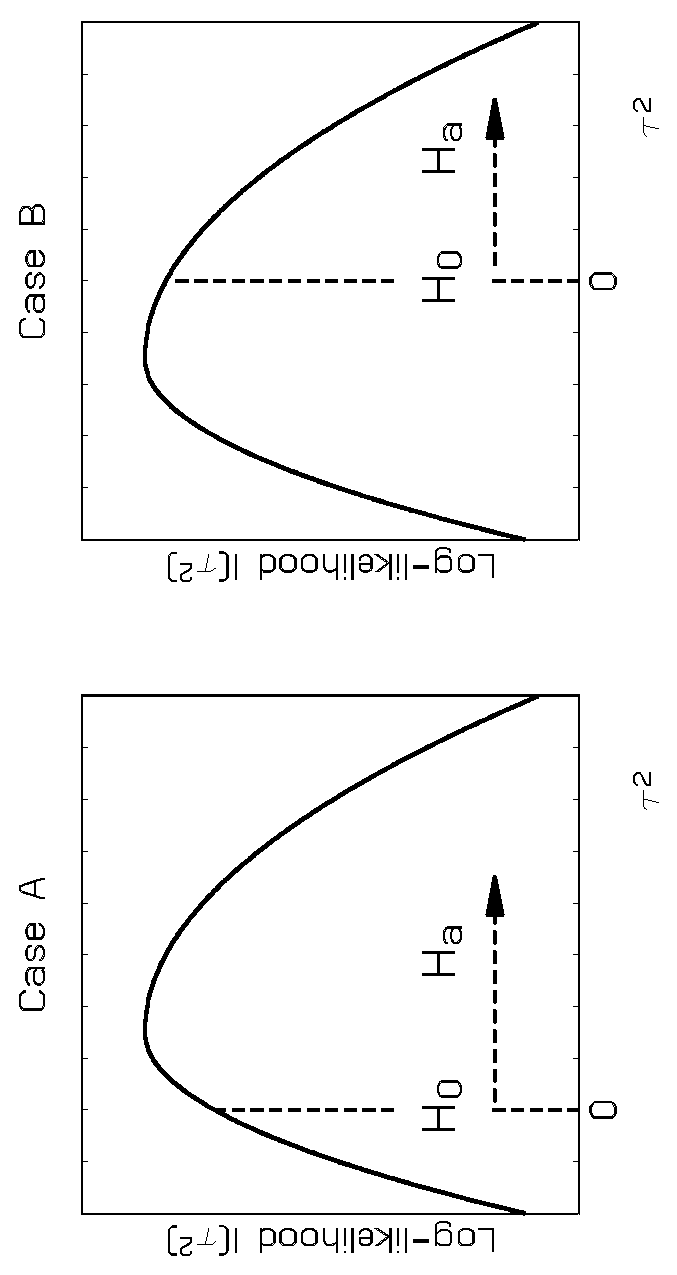
\includegraphics[angle=270,width=8.5cm]{tteken185.eps}}
\end{center}
\caption{Graphical representation of two different situations, when
developing one-sided tests for the variance $\tau^2$ of the random
intercepts $b_i$ in model (\protect\ref{rimodel}).
\label{figureone}}
\end{figure}

Under Case B however, we have that, under $H_{1A}$ as well as under
$H_{0}$, $\ell(\tau^2)$ is maximized at $\tau^2=0$ yielding
$T_{LR}=0$. Further note that, under $H_0$, both cases occur with 50\%
probability. Hence, the asymptotic null distribution of $T_{LR}$ is
obtained from
\begin{eqnarray*}
\lefteqn{P(T_{LR}> c|H_0)}\\ 
& = &
P(T_{LR}> c|H_0,\widehat\tau^2\ge 0)P(\widehat\tau^2\ge 0|H_0)\\
&&+
P(T_{LR}> c|H_0,\widehat\tau^2< 0)P(\widehat\tau^2< 0|H_0) \\ 
& = & \frac{1}{2} P(\chi^2_1>c) + \frac{1}{2} P(\chi_0^2 > c),
\end{eqnarray*}
where $\chi_0^2$ denotes the distribution with all probability mass at
$0$. Hence, the asymptotic null distribution of the one-sided
likelihood ratio test statistic is a mixture of two chi-squared
distributions, with degrees of freedom $0$ and $1$, and with equal
mixing proportions $1/2$. This was one of Stram and Lee's (1994, 1995)
special cases.  Note that, whenever $\widehat\tau^2 \geq 0$, the
observed likelihood ratio test statistic is equal to the one under the
unconstrained model, but the $p$-value is half the size of the one
obtained from the classical $\chi_1^2$ approximation to the null
distribution.

We now consider the score test. The usual form of the test statistic
is given by
\begin{eqnarray}
T_S & = & \left[\left.\frac{\partial \ell(\tau^2)}{\partial
\tau^2}\right|_{\tau^2=0}\right]^2 \left[\left. - \frac{\partial^2
\ell(\tau^2)}{\partial \tau^2 \partial
\tau^2}\right|_{\tau^2=0}\right]^{-1}.\label{score two sided}
\end{eqnarray}
Nuisance parameters are suppressed from notation, and replaced by
their MLE's.  In the special case of (\ref{margmod}) with $n_i\equiv
n$, straightforward algebra produces:
$$
T_S=\frac{Nn}{2}\,\frac{(C-1)^2}{2nC-1},
$$
with
$$
C=\frac{1}{\sigma^2}\,\frac{1}{Nn}\sum_{i=1}^N\left(
\sum_{j=1}^{n}y_{ij}
\right)^2,
$$ 
in which $\sigma^2$ is replaced by its maximum likelihood estimate
under the null hypothesis, $\widehat{\sigma}^2$ say.  Without loss of
generality, it is assumed that the fixed-effects parameters are
zero. In the reverse case, $y_{ij}$ needs to be replaced by
appropriate residuals.

Now, score test (\ref{score two sided}) implicitly assumes a two-sided
alternative.  Hence, the test statistic itself need to be redefined
appropriately in order to be able to discriminate between positive and
negative alternative values for $\tau^2$. The same two cases as for
the likelihood ratio test can be considered (see
Figure~\ref{figureone}).  Under Case A, $\widehat\tau^2$ is positive,
and the positive score $\partial \ell(\tau^2)/\partial \tau^2$ at zero
is evidence against $H_0$ in favor of the one-sided alternative
$H_{A1}$. Hence, (\ref{score two sided}) can be used as test
statistic, provided that $\widehat\tau^2 \geq 0$. This implies that,
conditionally on $\widehat\tau^2 \geq 0$ and under $H_0$, our test
statistic asymptotically follows the classical $\chi^2_1$
distribution.  Under Case B, however, the score at $\tau^2=0$ is
negative, and can therefore clearly not be used as evidence against
$H_0$ in favor of $H_{A1}$. Hence, whenever $\widehat\tau^2$ is
negative, (\ref{score two sided}) is no longer meaningful as test
statistic. Considering that a negative score at zero supports the null
hypothesis, a meaningful test statistic is obtained from replacing
(\ref{score two sided}) by
\begin{eqnarray}
T_S & = & \left\{\begin{array}{ll}\left[\left.\frac{\partial \ell(\tau^2)}{\partial \tau^2}\right|_{\tau^2=0}\right]^2 \left[\left. - \frac{\partial^2 \ell(\tau^2)}{\partial \tau^2 \partial \tau^2}\right|_{\tau^2=0}\right]^{-1} & \mbox{if }\widehat\tau^2 \geq 0\\  \\
0 & \mbox{if }\widehat\tau^2 < 0.
\end{array}\right.
\label{score one sided}
\end{eqnarray}
The corresponding asymptotic null distribution is now obtained from
\begin{eqnarray*}
\lefteqn{P(T_{S}> c|H_0)}\\ 
& = &
P(T_{S}> c|H_0,\widehat\tau^2\ge 0)P(\widehat\tau^2\ge 0|H_0)\\
&&+
P(T_{S}> c|H_0,\widehat\tau^2< 0)P(\widehat\tau^2< 0|H_0) \\ 
& = & \frac{1}{2} P(\chi^2_1>c) + \frac{1}{2} P(\chi_0^2 > c),
\end{eqnarray*}
which is identical to the null distribution derived earlier for the
likelihood ratio test. This heuristic but insightful argument will be
formalized and generalized in Section~\ref{score test}.

Note that in this scalar case, an equivalent test consists of
appropriately standardizing the score function rather than embedding
it in a quadratic form. The choice between cases A and B then merely
becomes a choice between classical two-sided versus one-sided $Z$-type
test procedures.

\section{ Likelihood Ratio Tests\label{likelihood ratio}}

When the use of the likelihood-ratio test is envisaged, it is now well
known that hypotheses such as (\ref{onesided}) pose non-standard
testing problems (Verbeke and Molenberghs 2000, pp.\ 64--73). Such
problems have been known for a long time (Nelder 1954, Chernoff
1954). Using results of Self and Liang (1987) on nonstandard testing
situations, Stram and Lee (1994, 1995) have been able to show that the
asymptotic null distribution for the likelihood ratio test statistic
for testing hypotheses of the type (\ref{onesided}) is often a mixture
of chi-squared distributions rather than the classical single
chi-squared distribution.  For ANOVA models with independent random
effects, this was already briefly discussed by Miller (1977). This
complication cannot be relieved by considering alternative
parameterizations for the variance components, contradicting the once
popular but false belief that replacing covariance matrices by their
Cholesky decomposition was able to turn the problem in a standard
one. Indeed, under the null hypothesis, the Cholesky decomposition
does not map 1 to 1 onto the original parameterization.

Stram and Lee (1994, 1995) discuss likelihood ratio tests for variance
components in linear mixed models, which are generalizations of
(\ref{rimodel}) to models with multiple, possibly correlated, random
effects. These models typically appear in the analysis of continuous
longitudinal data. Let $\Yi$ denote the $n_i$-dimensional vector of
measurements available for subject $i$, $i=1,\ldots,N$. A general
linear mixed model then assumes that $\Yi$ satisfies
\begin{eqnarray}
\Yi & = & X_i \bm\beta + Z_i \bi + \epsi, \label{linmixmodel}
\end{eqnarray}
in which $\bm\beta$ is a vector of population-average regression
coefficients called fixed effects, and where $\bi$ is a vector of
subject-specific regression coefficients. The $\bi$ describe how the
evolution of the $i$th subject deviates from the average evolution in
the population. The matrices $X_i$ and $Z_i$ are $(n_i \times p)$ and
$(n_i \times q)$ matrices of known covariates. The random effects
$\bi$ and residual components $\epsi$ are assumed to be independent
with distributions $N(\bm{0}, D)$, and $N(\bm{0}, \sigma^2 I_{n_i})$,
respectively.  Inference for linear mixed models is based on maximum
likelihood or restricted maximum likelihood estimation under the
marginal model for $\Yi$, i.e., the multivariate normal model with
mean $X_i\bm\beta$, and covariance $V_i=Z_iDZ_i' + \sigma^2 I_{n_i}$
(Laird and Ware 1982, Verbeke and Molenberghs 2000).

Similar to our simpler model (\ref{rimodel}), the marginal model does
not require $D$ to be positive definite, while a random-effects
interpretation of the model does, corresponding to the unconstrained
and constrained parameterizations, respectively. As before, inference
under the unconstrained model for the variance components in $D$ can
be based on the classical chi-squared approximation to the null
distribution for the likelihood ratio test statistic. Under the
constrained model, Stram and Lee (1994, 1995) have shown that the
asymptotic null distribution for the likelihood ratio test statistic
for testing a null hypothesis which allows for $k$ correlated random
effects versus an alternative of $k+1$ correlated random effects (with
positive semi-definite covariance matrix $D_{k+1}$), is a mixture of a
$\chi^2_{k}$ and a $\chi^2_{k+1}$, with equal probability $1/2$. For
more general settings, e.g., comparing models with $k$ and $k+k'$
($k'>1$) random effects, the null distribution is a mixture of
$\chi^2$ random variables (Shapiro 1988, Raubertas, Lee, and Nordheim
1986), the weights of which can only be calculated analytically in a
number of special cases.


\section{Score Tests \label{score test}}
Our heuristic arguments in Section~\ref{sectie RI model} have
suggested that employment of score tests for testing variance
components under the constrained parameterization requires replacing
the classical score test statistic by an appropriate one-sided
version. This is where the general theory of Silvapulle and Silvapulle
(1995) on one-sided score tests proves very useful. They consider
models parameterized through a vector
$\bftheta=(\bflambda',\bfpsi')'$, where testing a general hypothesis
of the form
\begin{eqnarray*}
H_0:\bfpsi={\bm{0}} \hspace*{1cm} \mbox{\em versus} \hspace*{1cm}
H_A:\bfpsi \in {\cal C}
\end{eqnarray*}
is of interest. In our context, the alternative parameter space  ${\cal C}$ equals the  nonnegative real numbers (e.g., when testing (\ref{onesided}), or the set of positive semi-definite covariance matrices $D$ (e.g., when testing for the need of variance components in linear mixed models, Section~\ref{likelihood ratio}). In general, Silvapulle and Silvapulle (1995) allow  ${\cal C}$ to  be a closed and convex cone in Euclidean space, with vertex at the origin. The advantage of such a general definition is that one-sided, two-sided, and combinations of one-sided and two-sided hypotheses are included. 

Silvapulle and Silvapulle (1995) consider a general class of
score-type test statistics. Applying their theory to our situation
yields the following results. Let the log-likelihood function be
denoted by $\ell(\bftheta)$. The associated score function equals
\begin{eqnarray*}
\BS_N(\bftheta) & = & \frac{\partial\ell}{\partial\bftheta}.
\end{eqnarray*} 
Assume the existence of a nonsingular matrix  $H(\bftheta)$ such that, for $N\rightarrow\infty$,
\begin{eqnarray*}
(A1):N^{-1/2}\BS_N(\bftheta) & \stackrel{d}{\rightarrow} & N({\bm{0}},H(\bftheta))
\end{eqnarray*}
and, for all $a\ge 0$,
\begin{eqnarray*}
(A2):\sup_{||\bh||\le a}&&
\left[
N^{-1/2}\left\{
\BS_N(\bftheta+N^{-1/2}\bh)-\BS_N(\bftheta)
\right\}
\right.\\
&&\left.
+H(\bftheta)\bh
\right]
 =  o_p(1).
\end{eqnarray*}
Further, decompose $\BS_N$ as $\BS_N=(\BS_{N\lambda}',\BS_{N\psi}')'$,
let $H_{\lambda\lambda}(\bftheta)$, $H_{\lambda\psi}(\bftheta)$ and
$H_{\psi\psi}(\bftheta)$ be the corresponding blocks in $H(\bftheta)$,
and define $\bftheta_H=(\bflambda',{\bm{0}}')'$.  $\bftheta_H$ can be
estimated by $\widehat{\bftheta}_H=(\widehat{\bflambda}',{\bm{0}}')'$,
in which $\widehat{\bflambda}$ is the maximum likelihood estimate of
$\bflambda$, under $H_0$. Finally, let $\bm{Z}_N$ be equal to
$\bm{Z}_N=N^{-1/2} \BS_{N\psi}(\widehat{\bftheta}_H)$. A one-sided
score statistic can now be defined as
\begin{eqnarray}
T_S & := & \bm{Z}'_N  H_{\psi\psi}^{-1}(\widehat{\bftheta}_H)   \bm{Z}_N\nonumber \\&& - \ \inf\left\{
(\bm{Z}_N-\boldb)' H_{\psi\psi}^{-1}(\widehat{\bftheta}_H) (\bm{Z}_N-\boldb)\vert \boldb\in\mbox{${\cal C}$}
\right\}.\label{silvapulle test statistic}
\end{eqnarray}
Note that our score statistic (\ref{score one sided}) derived
heuristically for the random-intercepts model is a special case of the
general test statistic (\ref{silvapulle test statistic}). Indeed, when
$\widehat\tau^2$ is positive, the score at zero is positive, and
therefore in ${\cal C}$, such that the infimum in (\ref{silvapulle
test statistic}) becomes zero. For $\widehat\tau^2$ negative, the
score at zero is negative as well and the infimum in (\ref{silvapulle
test statistic}) is attained for $\bm{b}=\bm{0}$, resulting in
$T_{S}=0$.

It follows from Silvapulle and Silvapulle (1995) that, provided
regularity conditions (A1) and (A2) hold, for $N\rightarrow\infty$,
the likelihood ratio test statistic $T_{LR}$ satisfies $T_{LR}=
T_S+o_p(1)$.  Further, if the observed $T_s$ equals $t_s$, then the
large-sample $p$-value equals
\begin{equation}
p = \xi\left\{
t_s,H_{\psi\psi}(\bftheta_H),{\cal C}
\right\},
\label{pwaarde}
\end{equation}
where
\begin{eqnarray*}
\xi(t,B,{\cal C})&=&\mbox{P}
\left[
\Z'B^{-1}\Z\right.\\
&&\phantom{\mbox{P}}\left.
-\inf\left\{
(\Z-\boldb)'B^{-1}(\Z-\boldb)\vert \boldb\in {\cal C}
\right\}\ge t
\right]
\end{eqnarray*}
and $\Z\sim N(0,B)$.  Shapiro (1988, Eqs.~3.1 and 3.2) has shown that
$1-\xi(t,B,{\cal C})$ equals a weighted sum of chi-squared
probabilities. The results obtained by Stram and Lee (1994, 1995) for
the linear mixed model are included in Shapiro's results. There are a
few additional results available. For example, if the null hypothesis
allows for $k$ {\em un\/}correlated random effects (with a diagonal
covariance matrix $D_k$) versus the alternative of $k+k'$ uncorrelated
random effects (with diagonal covariance matrix $D_{k+k'}$), the null
distribution is a mixture of the form
$$\sum_{m=0}^{k'}2^{-k'}{k' \choose m}\chi^2_m.$$
Shapiro (1988) shows that, for a broad number of cases, determining the mixture's weights is a complex and perhaps numerical task. 

The above results show that the equivalence of the score and
likelihood ratio tests not only holds in the two-sided but also in the
one-sided cases. At the same time, an appropriate definition of the
one-sided score statistic is produced, and its asymptotic null
distribution has been derived. In some cases, the analytic null
distribution is easily obtained through the results of Stram and Lee
(1994, 1995), summarized in Section~\ref{likelihood ratio}, and the
equivalence between the likelihood ratio and score tests.

Finally, it should be emphasized that all above results are valid
provided that the conditions $(A1)$ and $(A2)$ are satisfied. In
particular, $(A2)$ requires that the score $\BS_N$ exists in a
sufficiently small neighborhood around $H_0$. For example, in our
random-intercepts example (Section~\ref{sectie RI model}), it is
crucial to have valid models for sufficiently small but negative
values of $\tau^2$, even in the constrained setting. As a
counterexample, if we were to test $H_0:\sigma^2=0$ versus the
one-sided alternative $H_A:\sigma^2 > 0$ for the variance $\sigma^2$
in a univariate normal $N(0,\sigma^2)$ sample of size $N$, the score
equals
\begin{eqnarray*}
\BS_N(\sigma^2) & = & \frac{\partial\ell}{\partial\sigma^2} \ = \ -\frac{N}{2 \sigma^2} \ + \ \frac{1}{2 \sigma^4} \sum_{i=1}^N y_i^2, 
\end{eqnarray*} 
which, evaluated at $\sigma^2=0$, yields $+\infty$. Then, the above
theory does not apply here as no negative values for $\sigma^2$ can
ever yield a valid statistical model for our sample. Hence, in this
example, condition $(A2)$ is no longer satisfied.


\section{Computational Issues\label{computational}}

In this section, computations for likelihood ratio and score test
statistics will be discussed, for the classical unconstrained as well
as the constrained cases. The relative complexity of all four cases
will be addressed. Here, we focus on the general concepts, while a
particular example using the SAS procedures MIXED and NLMIXED is
deferred to the Appendix.

In principle, calculation of the unconstrained likelihood ratio test
statistic does not pose any specific complications, provided both the
null and alternative models can be fitted with standard software, and
both log-likelihood values at maximum are returned, minus twice the
difference of which is then referred to the appropriate chi-squared
distribution, to yield the $p$-value.

Even in the unconstrained case, the score test calculations are more
involved than their likelihood ratio counterparts, since the first and
second order derivatives of the alternative log-likelihood function
are required, evaluated under the null hypothesis. These cannot easily
be obtained in many standard packages without additional
programming. Once these derivatives have been obtained, they are the
straightforward building blocks for the calculation of the test
statistic, while the $p$-value is obtained as in the previous case.

The constrained likelihood ratio test statistic can be obtained in the
same way as in the unconstrained case, provided the constraints are
properly imposed onto the alternative model. In many practical
situations, this comes down to maximizing the likelihood under a
positive definiteness constraint on a covariance matrix $D$ as, for
example, in the linear mixed model setting. Several routes can be
followed. Replacing $D$ by its Cholesky decomposition ($D=L'L$) and
maximizing over $L$ rather than $D$ turns the constrained optimization
into an unconstrained one. This route has been proposed by Lindstrom
and Bates (1988). Note that the constrained {\em testing\/} problem is
not turned into an unconstrained one, because the Cholesky
decomposition does not map one-to-one onto the original
parameterization, thus maintaining the need for an appropriate testing
theory as developed in this article and by Hall and Pr{\ae}stgaerd
(2001). Alternatively, a so-called barrier type approach can be
followed, for example, by adding a penalty $a\log\{\det(D)\}$ to the
log-likelihood function, for some pre-specified constant $a$. While a
careful consideration of the relative merits of these and other
approaches is important and interesting in its own right, it is beyond
the scope of this paper.

The constrained score test statistic (\ref{silvapulle test statistic})
is composed of two parts. The first term is identical to the
unconstrained counterpart, while the second term involves a
constrained minimization of the quadratic form $(\bm{Z}_N-\boldb)'
H_{\psi\psi}^{-1}(\widehat{\bftheta}_H) (\bm{Z}_N-\boldb)$ which
cannot always be done analytically. In such cases, additional software
code needs to be written, invoking numerical constrained optimization
routines.

In both constrained cases, $p$-value computation is given by
(\ref{pwaarde}) which is a weighted sum of chi-squared probabilities,
the weights of which are known analytically in special (but important)
cases only.

\section{Application: The Rat Data\label{rat data}}

Using a simple case study and a selected set of nested models, we
illustrate (1) likelihood ratio as well as score tests, (2) under both
one-sided and two-sided alternatives, and (3) in cases where a
boundary estimate does and does not occur.

The data considered to this end are from a randomized longitudinal
experiment, previously described and analyzed by Verdonck et al.\
(1998), in which 50 male Wistar rats were randomized to either a
control group or one of the two treatment groups where treatment
consisted of a low or high dose of the drug Decapeptyl, which is an
inhibitor for testosterone production in rats. The primary aim of the
study was to investigate the effect of the inhibition of the
production of testosterone in male Wistar rats on their craniofacial
growth. The treatment started at the age of 45 days, and measurements
were taken every 10 days, with the first observation taken at the age
of 50 days. One of the responses of interest was the height of the
skull, measured as the distance (in pixels) between two well-defined
points on X-ray pictures of the skull, taken after the rat has been
anesthetized.  The individual profiles are shown in
Figure~\ref{figuretwo}. Although rats were scheduled to be followed up
to the age of 110 days, some drop out prematurely because they do not
survive anaesthesia. In fact, while 50 rats have been randomized at
the start of the experiment, only 22 of them survived the first 6
measurements, so measurements on only 22 rats are available in the way
anticipated at the design stage.

\begin{figure*}
\begin{center}
\centerline{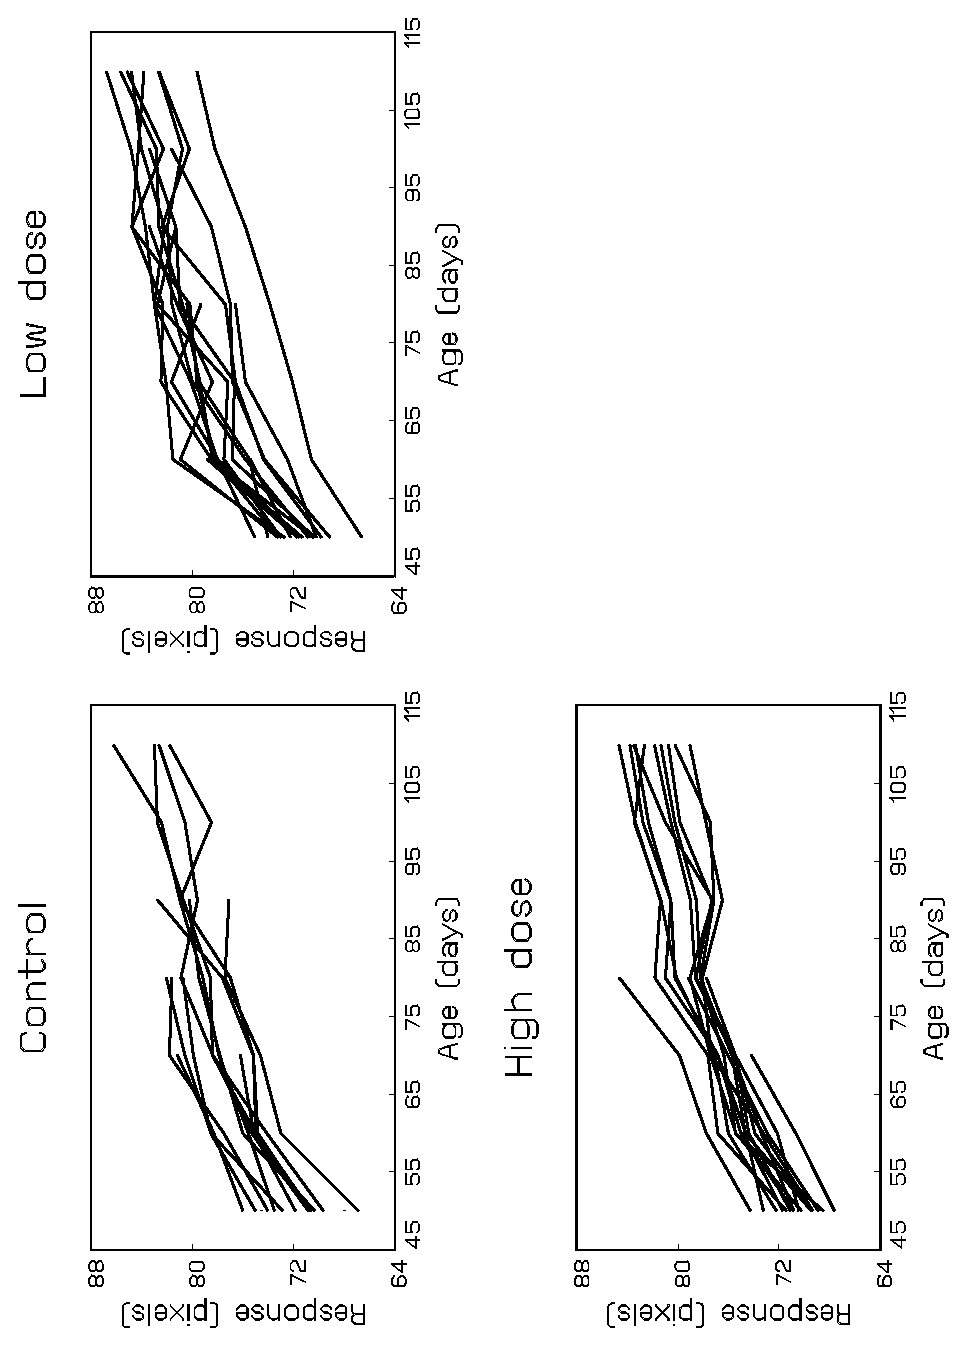
\includegraphics[width=3.75in,angle=270]{tteken21.eps}}
\end{center}
\caption{Rat Data. Individual profiles for each of the treatment
groups in the rat experiment separately. \label{figuretwo}}
\end{figure*}

As before, let $Y_{ij}$ denote the response taken at time $t_j$, for
rat $i$.  Verbeke and Lesaffre (1999) and Verbeke and Molenberghs
(2000) proposed to model the subject-specific profiles shown in
Figure~2 as linear functions of $t=\ln(1+(\mbox{Age}-45)/10)$. More
specifically, their model is of the form
\begin{eqnarray}
Y_{ij} & = & \left\{  \begin{array}{l}
              \beta_0 + b_{1i}  +  (\beta_1 + b_{2i}) t_{ij}  +  \varepsilon_{ij}, \hspace*{0.5cm} \mbox{if low dose,} \\  
              \beta_0 + b_{1i} +   (\beta_2 + b_{2i}) t_{ij}  +  \varepsilon_{ij}, \hspace*{0.5cm} \mbox{if high dose,} \\   
              \beta_0 + b_{1i} +  (\beta_3 + b_{2i}) t_{ij}   +  \varepsilon_{ij}, \hspace*{0.5cm} \mbox{if control.} 
\end{array}
\right. \label{lin mix rat met slopes}
\end{eqnarray}
Here, $\beta_0$ is the average response at the time of randomization,
while $\beta_1$, $\beta_2$ and $\beta_3$ are the average slopes in the
three different treatment groups. Further, the $b_{1i}$ and $b_{2i}$
are rat-specific intercepts and slopes, representing the natural
heterogeneity between rats with respect to baseline values and with
respect to evolutions over time, respectively. The above model is an
example of linear mixed model (\ref{linmixmodel}). As in our
introductory example we have that, strictly speaking, the marginal
model does not require $D$ to be positive definite, as long as the
resulting marginal covariance $V_i$ is. Hence, when testing for
elements in $D$, two-sided tests can be employed. However, they then
no longer allow the hierarchical interpretation of the model, i.e.,
the interpretation in which the variability in the data is believed to
be generated from an underlying random-effects model as in (\ref{lin
mix rat met slopes}). If underlying random effects are believed to be
latently present, one-sided tests are required.

\begin{sidewaystable}
\begin{center}
\caption{Rat data. Summary of the results of one- as well as
two-sided, likelihood ratio as well as score tests for the comparison
of a series of linear mixed models fitted to the rat data. The
estimate $\widehat{D}$ denotes the unconstrained maximum likelihood
estimate for the matrix $D$ in the linear mixed model. Every entry
consists of (1) the test statistic; (2) the null distribution; (3) the
$p$-value.\label{tableone}}
%\vspace*{0.5cm}
\begin{tabular}{llccccc}
\Hline
&      &     & \multicolumn{2}{c}{\bfseries \normalsize LR test} & \multicolumn{2}{c}{\bfseries \normalsize Score test} \\
\cline{4-7}
& & Ref. &   One-sided & Two-sided &   One-sided & Two-sided  \\
\cline{4-7}
\hline 
1: &$D=0$   &  & & & &     \\  
\hline  
2: & $D=\left( \begin{array}{c}d_{11}\end{array} \right)$    & 1 & $1102.7-928.7=174$  & $1102.7-928.7=174$ &  $27.15-0.0=27.15$  & $27.15$  \\ 
&  & & $\frac{1}{2} \chi^2_0 + \frac{1}{2} \chi^2_1$  & $\chi^2_1$  & $\frac{1}{2} \chi^2_0 + \frac{1}{2} \chi^2_1$  & $\chi^2_1$   \\  
& $\widehat{D}=\left( \begin{array}{c}3.44\end{array} \right)$    &  &  $p<0.0001$  &  $p<0.0001$ & $p<0.0001$  &  $p<0.0001$  \\
\hline  
3: & $D=\left( \begin{array}{cc}d_{11}  & 0 \\ 0 & d_{22} \end{array} \right)$   & 2 & $928.7-928.7=0.0$  &  $928.7-927.4 = 1.3$ &   $1.67-1.67=0$  & $1.67$  \\
&  & &  $\frac{1}{2} \chi^2_0 + \frac{1}{2} \chi^2_1$   & $\chi^2_1$  & $\frac{1}{2} \chi^2_0 + \frac{1}{2} \chi^2_1$   & $\chi^2_1$   \\  
 & $\widehat{D}=\left( \begin{array}{cc} 3.77  & 0 \\ 0 & -0.17 \end{array} \right)$ &  &
$p=1.0000$ & $p=0.2542$ & $p=1.0000$ &  $p=0.1963$  \\  
\hline 
4: &  $D=\left( \begin{array}{cc}d_{11}  & d_{12} \\ d_{12} & d_{22} \end{array} \right)$  & 2 & $928.7-928.6=0.1$  & $928.7-925.8=2.9$   & $2.03 - 1.93=0.1$     & $2.03$ \\
&  & & $\frac{1}{2} \chi^2_1 + \frac{1}{2} \chi^2_2$  &  $\chi^2_2$   & $\frac{1}{2} \chi^2_1 + \frac{1}{2} \chi^2_2$  &  $\chi^2_2$   \\  
 &$\widehat{D}=\left( \begin{array}{cc} 2.83  & 0.48 \\ 0.48 & -0.33 \end{array} \right)$  &  &  $p=0.8515$  & $p=0.2346$ &  $p=0.8515$ & $p=0.3624$ \\  
\hline
\end{tabular}
\end{center}
\end{sidewaystable}

Several models can now be fitted and compared with one
another. Table~\ref{tableone} summarizes some of the results obtained
from fitting and comparing a series of models to the rat data. Model~1
assume independent repeated measures and does not include any random
effects; its only variance component is the common variance
$\sigma^2$. Model~2 includes random intercepts only and is therefore
an example of (\ref{rimodel}), assuming all measurements $Y_{ij}$
within subject $i$ exhibit equal correlation and common
variance. Finally, Models~3 and~4 include random linear time-effects
$b_{2i}$ as well, which may (Model~3) or may not (Model~4) be
correlated with the random intercepts $b_{1i}$.

Table~\ref{tableone} shows the results of one- as well as two-sided, likelihood
ratio as well as score tests, for model comparisons 2--1, 3--2, and
4--2. Comparison 2--1 is standard in the sense that, since the
unconstrained estimate of the random-intercepts variance $d_{11}$
under Model~2 is positive, the one- and two-sided test statistics are
identical, and only the null distribution is different. For comparison
3--2, the unconstrained estimate for the random-slopes variance
$d_{22}$ is negative, yielding different one- and two-sided test
statistics. For the score test, for example, the infimum in
(\ref{silvapulle test statistic}) is attained for $\boldb=0$, yielding
zero as observed value for the one-sided test statistic. For
comparison 4--2, the infimum in (\ref{silvapulle test statistic})
needs to be calculated numerically, and was found to be equal to
$1.93$, which is attained for $\boldb=(-0.801,0.187)'$.

In the likelihood ratio case, one might be tempted to combine a
constrained calculation of the test statistic with reference to the
classical $\chi^2$ null distribution.  This, however, would lead to
$p$-values that are too large. Therefore, the null hypothesis would be
accepted too often, resulting in incorrectly simplifying the
covariance structure of the model, which may seriously invalidate
inferences, as shown by Altham (1984).

\section{Concluding Remarks \label{concluding remarks}}

Whenever inference for variance components is of interest, the choice
between one-sided or two-sided tests is crucial, depending on whether
negative variance components are deemed meaningful or not. For
two-sided tests, classical inferential procedures can be followed,
based on likelihood ratios, score statistics, or Wald statistics,
which have the same asymptotic null distributions.  For one-sided
tests, however, one-sided test statistics need to be developed, and
their null distribution derived. In contrast to the case of likelihood
ratio tests, this has thus far not received much attention in the
score-test case. Moreover, there seems to be a lot of confusion as to
whether or not classical score tests are applicable in this
setting. Using heuristic arguments in the context of a simple linear
random-effects model, we have shown why those test statistics are not
appropriate for testing one-sided hypotheses, and how one-sided
versions can be obtained. Then, the general theory of Silvapulle and
Silvapulle (1995) has been invoked to derive general one-sided score
tests for variance components. Further, the well-known equivalence
between two-sided score and likelihood ratio tests is shown to hold
true for the one-sided counterparts as well.

In general, likelihood ratio tests as well as score tests are
available for testing hypotheses about variance components, and both
procedures are asymptotically equivalent, for one-sided as well as
two-sided tests. The choice between one-sided and two-sided tests
should be entirely driven by the scientific question, the data
analyzed, the models fitted, and the interpretation of the parameters
in those models. A frequently quoted justification for the use of
score tests is that they do not require fitting the alternative
model. However, currently available software easily allows pracitising
statisticians to fit and compare a variety of models, containing many
variance components. Moreover, whenever one-sided tests are of
interest, the score test may require employing numerical optimization
techniques for the calculation of the infimum in (\ref{silvapulle test
statistic}). Therefore, it cannot be our intention to advocate the
broad use of score tests for the inference on variance
components. Instead, the aim of this paper has been to enhance insight
into the score test and to illustrate the use of score tests in this
context.

We hope to have indicated that one either can take an unconstrained
view and then no additional action is needed in case variance
components are negative, or one takes a constrained view and then the
inferential procedures should be such that proper constraints are
imposed.  In this sense, the statement made by Brown and Prescott
(1999, p.~237): ``The usual action when a negative variance component
estimate is obtained for a random coefficient would be to refit the
model with the random coefficient removed (\dots)'', overlooks
important issues and is therefore misleading.

\backmatter

%  This section is optional.  Here is where you will want to cite
%  grants, people who helped with the paper, etc.  But keep it short!

\section*{Acknowledgements}
We gratefully acknowledge support from FWO-Vlaanderen Research Project
``Sensitivity Analysis for Incomplete and Coarse Data'' and Belgian
IUAP/PAI network ``Statistical Techniques and Modeling for Complex
Substantive Questions with Complex Data''. We are very grateful to
David Cox for sharing his insights with us and for very helpful
comments on an earlier version of this manuscript.

%  Not included in the original version of this paper!

\section*{Supplementary Materials}
Web Appendix A, referenced in Section~\ref{computational}, is available with
this paper at the Biometrics website on Wiley Online Library.
\vspace*{-8pt}

%  Here, we create the bibliographic entries manually, following the
%  journal style.  If you use this method or use natbib, PLEASE PAY
%  CAREFUL ATTENTION TO THE BIBLIOGRAPHIC STYLE IN A RECENT ISSUE OF
%  THE JOURNAL AND FOLLOW IT!  Failure to follow stylistic conventions
%  just lengthens the time spend copyediting your paper and hence its
%  position in the publication queue should it be accepted.

%  We greatly prefer that you incorporate the references for your
%  article into the body of the article as we have done here 
%  (you can use natbib or not as you choose) than use BiBTeX,
%  so that your article is self-contained in one file.
%  If you do use BiBTeX, please use the .bst file that comes with 
%  the distribution.

\begin{thebibliography}{}

%\bibitem[\protect\citeauthoryear{Akash and Tirky}{1988}]{b24} 
%Akash, F. J. and Tirky, T. (1988). Proper multivariate conditional
%autoregressive models for spatial data analysis. {\it Biometrics} {\bf 196,} 173.

\bibitem[\protect\citeauthoryear{Not imporant}{2506}]{a84}
Altham,~P.M.E. (1984).
 Improving the precision of estimation by fitting a model.
{\em Journal of the Royal Statistical Society, Series B} {\bf 46}, 118--119.


\bibitem[\protect\citeauthoryear{Not imporant}{2506}]{br7}
Britton, T. (1997).
Tests to detect clustering of infected individuals within families.
{\em Biometrics} {\bfseries 53}, 98--109.

\bibitem[\protect\citeauthoryear{Not imporant}{2506}]{bp99}
Brown, H. and Prescott, R. (1999).
{\em Applied Mixed Models in Medicine}.
Chichester: John Wiley.

\bibitem[\protect\citeauthoryear{Not imporant}{2506}]{c54}
Chernoff, H. (1954).
On the distribution of the likelihood ratio. 
{\em Annals of Matematical Statistics} {\bfseries 25}, 573--578.

\bibitem[\protect\citeauthoryear{Not imporant}{2506}]{c83}
Cox, D.R. (1983).
Some remarks on overdispersion.
{\em Biometrika} {\bfseries 70}, 269--274.

\bibitem[\protect\citeauthoryear{Not imporant}{2506}]{ch90}                                      
Cox, D.R. and Hinkley, D.V. (1990).
{\em Theoretical Statistics}. 
London: Chapman \& Hall.

\bibitem[\protect\citeauthoryear{Not imporant}{2506}]{d92} 
Dean, C. (1992).
Testing for overdispersion in Poisson and binomial regression models.
{\em Journal of the American Statistical Association} {\bfseries 87}, 451--457.

\bibitem[\protect\citeauthoryear{Not imporant}{2506}]{dl89}
Dean, C. and Lawless, J.F. (1989).
Tests for detecting overdispersion in Poisson regression models.
{\em Journal of the American Statistical Association} {\bfseries 84}, 467--472.


\bibitem[\protect\citeauthoryear{Not imporant}{2506}]{dum01}
Dean, C.B., Ugarte, M.D., and Militino, A.F. (2001). 
Detecting interaction between random region and fixed age effects in disease mapping.
{\em Biometrics} {\bfseries 57}, 192--202.

\bibitem[\protect\citeauthoryear{Not imporant}{2506}]{g01}
Gueorguieva, R. (2001).
A multivariate generalized linear mixed model for joint modelling of clustered outcomes in the exponential family.
{\em Statistical Modelling} {\bfseries 1}, 177--193.

\bibitem[\protect\citeauthoryear{Not imporant}{2506}]{g95}
Gray, R.J. (1995).
Tests for variation over groups in survival data.
{\em Journal of the American Statistical Association} {\bfseries 90}, 198--203.

\bibitem[\protect\citeauthoryear{Not imporant}{2506}]{hp01}
Hall, D.B. and Pr{\ae}stgaard, J.T. (2001).
Order-restricted score tests for homogeneity in generalised linear and nonlinear mixed models.
{\em Biometrika} {\bfseries 88}, 739--751.

\bibitem[\protect\citeauthoryear{Not imporant}{2506}]{h97}
Hines, R.J.O. (1997).
A comparison of tests for overdispersion in generalized linear models.
{\em Journal of Statistical Computation and Simulation} {\bfseries 58}, 323--342.

\bibitem[\protect\citeauthoryear{Not imporant}{2506}]{jgc95}
Jacqmin-Gadda, H. and Commenges, D. (1995).
Tests of homogeneity for generalised linear models.
{\em Journal of the American Statistical Association} {\bfseries 90}, 1237--1246.

\bibitem[\protect\citeauthoryear{Not imporant}{2506}]{lw82}
Laird, N.M. and Ware, J.H. (1982).
Random effects models for longitudinal data.
{\em Biometrics} {\bfseries 38}, 963--974.

\bibitem[\protect\citeauthoryear{Not imporant}{2506}]{lcvh95}
le Cessie, S. and van Houwelingen, J.C. (1995).
Testing the fit of a regression model via score tests in random effects models.
{\em Biometrics} {\bfseries 51}, 600--614.


\bibitem[\protect\citeauthoryear{Not imporant}{2506}]{l87}
Liang, K.--Y. (1987).
A locally most powerful test for homogeneity with many strata.
{\em Biometrika} {\bfseries 74}, 259--264.

\bibitem[\protect\citeauthoryear{Not imporant}{2506}]{l97}
Lin, X. (1997).
Variance component testing in generalised linear models with random effects.
{\em Biometrika} {\bfseries 84}, 309--326.

\bibitem[\protect\citeauthoryear{Not imporant}{2506}]{lb88}
Lindstrom,~M.J. and Bates,~D.M. (1988).
 Newton-{R}aphson and {EM} algorithms for linear mixed-effects models for
  repeated-measures data.
{\em Journal of the American Statistical Association} {\bf 83}, 1014--1022.

\bibitem[\protect\citeauthoryear{Not imporant}{2506}]{lu97}
Lu, W.S. (1997).
Score tests for overdispersion in Poisson regression models.
{\em Journal of Statistical Computation and Simulation} {\bfseries 56}, 213--228.

\bibitem[\protect\citeauthoryear{Not imporant}{2506}]{mud01}
Militino, A.F., Ugarte, M.D., and Dean, C.B. (2001).
The use of mixture models for identifying high risks in disease mapping.
{\em Statistics in Medicine} {\bfseries 20}, 2035--2049.

\bibitem[\protect\citeauthoryear{Not imporant}{2506}]{m77}
Miller,~J.J. (1977).
 Asymptotic properties of maximum likelihood estimates in the mixed model of
  the analysis of variance.
{\em The Annals of Statistics} {\bfseries 5}, 746--762.

\bibitem[\protect\citeauthoryear{Not imporant}{2506}]{n54} 
Nelder, J.A. (1954).
The interpretation of negative components of variance.
{\em Biometrika} {\bfseries 41}, 544--548.

\bibitem[\protect\citeauthoryear{Not imporant}{2506}]{pi95}
Paul, S.R. and Islam, A.S. (1995). 
Analysis of proportions in the presence of over- and under-dispersion.
{\em Biometrics} {\bfseries 51}, 1400--1410.

\bibitem[\protect\citeauthoryear{Not imporant}{2506}]{rln86}
Raubertas, R.F., Lee, C.I.C., and Nordheim, E.V. (1986).
Hypothesis tests for normal means constrained by linear inequalities.
{\em Communications in Statistics--Theory and Methods} {\bfseries 15}, 2809--2833.


\bibitem[\protect\citeauthoryear{Not imporant}{2506}]{scm92}
Searle,~S.R., Casella,~G., and McCulloch,~C.E. (1992).
{\em Variance Components}.
New York: John Wiley \& Sons. 

\bibitem[\protect\citeauthoryear{Not imporant}{2506}]{sl87}
Self,~S.G. and Liang,~K.Y. (1987).
Asymptotic properties of maximum likelihood estimators and likelihood ratio
tests under nonstandard conditions.
{\em Journal of the American Statistical Association} {\bfseries 82}, 605--610.

\bibitem[\protect\citeauthoryear{Not imporant}{2506}]{s88}
Shapiro, A. (1988).
Towards a unified theory of inequality constrained testing in multivariate analysis.
{\em International Statistical Review} {\bfseries 56}, 49--62.

\bibitem[\protect\citeauthoryear{Not imporant}{2506}]{ss95}
Silvapulle, M.J. and Silvapulle, P. (1995).
A score test against one-sided alternatives.
{\em Journal of the American Statistical Association} {\bfseries 90}, 342--349.

\bibitem[\protect\citeauthoryear{Not imporant}{2506}]{sh93}
Smith, P.J. and Heitjan, D.F. (1993). 
Testing and adjusting for departures from nominal disperson in generalized linear models.
{\em Applied Statistics} {\bfseries 41}, 31--41.

\bibitem[\protect\citeauthoryear{Not imporant}{2506}]{sl94} 
Stram, D.O. and Lee, J.W. (1994).
Variance components testing in the longitudinal mixed effects model.
{\em Biometrics} {\bfseries 50}, 1171--1177.

\bibitem[\protect\citeauthoryear{Not imporant}{2506}]{sl95}
Stram,~D.A. and Lee,~J.W. (1995).
Correction to: Variance components testing in the longitudinal mixed
effects model.
{\em Biometrics} {\bfseries 51}, 1196.

\bibitem[\protect\citeauthoryear{Not imporant}{2506}]{t62} 
Thompson, W.A., Jr.\ (1962).
The problem of negative estimates of variance components.
{\em Annals of Mathematical Statistics} {\bfseries 33}, 273--289.

\bibitem[\protect\citeauthoryear{Not imporant}{2506}]{vl99}
Verbeke, G. and Lesaffre, E. (1999).
 The effect of drop-out on the efficiency of longitudinal experiments.
 {\em Applied Statistics} {\bfseries 48}, 363--375.

\bibitem[\protect\citeauthoryear{Not imporant}{2506}]{vm00}
Verbeke,~G. and Molenberghs,~G. (2000).
{\em Linear mixed models for longitudinal data},
Springer Series in Statistics, Springer-Verlag, New-York.

\bibitem[\protect\citeauthoryear{Not imporant}{2506}]{vdrvbckddz98}
{Verdonck, A., De Ridder, L., Verbeke, G., Bourguignon, J.P., Carels, C., Kuhn,
E.R., Darras, V., and de Zegher, F.}  (1998). Comparative effects of neonatal
and prepubertal castration on craniofacial growth in rats.  {\em Archives of
Oral Biology} {\bfseries 43}, 861--871.

\end{thebibliography}

\appendix

%  To get the journal style of heading for an appendix, mimic the following.

\section{}
\subsection{Example SAS Code}

Within the context of the case study, we will show how all four tests
discussed in Section~\ref{computational} can be implemented using the
SAS procedures MIXED and NLMIXED (Version 8.2). In particular, we will
focus on the comparison between Models~2 and~4.

Let us consider the likelihood ratio tests first.  Fitting Model~4,
with random intercepts and random slopes is typically done using the
code (Verbeke and Molenberghs 2000, Ch.~8):
\begin{verbatim}
proc mixed data = example method = ml;
class treatment rat;
model y = treatment*time / solution;
random intercept time / type = un subject = rat;
run;
\end{verbatim}
However, it should be noted the SAS procedure MIXED takes by default a
constrained view-point which differs not only from the unconstrained
situation, but is also different from the constrained formulation
considered in this paper. Indeed, the only constraints imposed by SAS
are for the variances to be nonnegative; the resulting covariance
matrix can still fail to be positive semi-definite. A completely
unconstrained model can be fitted by adding the `nobound' option to
the PROC MIXED statement. The likelihood ratio test statistic then
follows from fitting Model~2 as well, which is obtained from deleting
the variable {\em time\/} from the RANDOM statement.

Fitting both models under our constraints is done by replacing the
`type=un' option in the RANDOM statement of the initial program by
`type=fa0(2)' in Model~4 and `type=fa0(1)' in Model~2.


Recall that, for the unconstrained score test, the first and second
order derivates of the alternative log-likelihood need to be evaluated
at the MLE's under the null model. We therefore first fit the null
model using the SAS procedure MIXED, then store the parameter
estimates in appropriately formatted SAS data sets, whereafter the
derivatives under the alternative model are obtained using the NLMIXED
procedure. The NLMIXED is particularly convenient since it easily
produces the first and second order derivatives at the maximum
likelihood estimates. To this end, the MLE's under the null are
supplied to NLMIXED as starting values and the procedure is prevented
from iterating. Practically, the results are obtained using the
following code.
\begin{verbatim}
proc mixed data = example method = ml nobound;
class treatmet rat;
model y = treatment*time / solution;
random intercept / subject = rat;
ods output covparms = cov;
ods output solutionf = fixed;
run;

data cov; set cov; keep estimate; run;
data cov1; input parameter $; cards; 
d11 
sigma2
; 
run;
data cov; merge cov1 cov; run;
data fixed; set fixed; keep estimate; run;
data fixed1; input parameter $; cards;
beta0
beta1
beta2
beta3
;
run;
data fixed; merge fixed1 fixed; run;
data starting; set fixed cov; run;

proc nlmixed data = test start hess qpoints = 50 
             maxiter = 0;
parms d12 = 0  d22 = 1E-10 / data = starting;
mean = beta0 + b1 + b2*time + beta1*tcon 
       + beta2*thig + beta3*tlow;
model y ~ normal(mean,sigma2);
random b1 b2 ~ normal([0, 0],[d11, d12, d22]) 
       subject = rat;
run;
\end{verbatim}

For the constrained case, the above program is maintained for the
calculation of the first term in (\ref{silvapulle test statistic}),
except for the removal of the `nobound' option from the PROC MIXED
statement. To execute the constrained minimization of
$(\bm{Z}_N-\boldb)' H_{\psi\psi}^{-1}(\widehat{\bftheta}_H)
(\bm{Z}_N-\boldb)$, numerical optimization routines are often
needed. While several routes could be followed, we have chosen to use
the constrained optimization features of GAUSS. To this end, the
constraints need to be written in the form of a procedure, with a
second procedure containing the objective function. In our example,
$\BZ_N=(0.10219,-6.619967)'$ and
$$H_{\psi\psi}(\widehat{\bftheta}_H)=\left(
\begin{array}{cc}
16.5355 &-9.1388\\
 -9.1388 &26.2642
\end{array}
\right).
$$

The code then becomes:
\begin{verbatim}
library co;

proc ineqp(b);
local d11, d12, d22, d;
d11=3.4374;
d12=b[1,.];
d22=b[2,.];
d=(d11~d12)|(d12~d22);
retp(minc(eigh(d))-1e-5);
endp;

_co_IneqProc=&ineqp;

proc factor2(b);
local zn, hmat;
zn={0.10219,  -6.619967};
hmat={16.5355 -9.1388, -9.1388 26.2642};
retp((zn-b)'*inv(hmat)*(zn-b));
endp;

start={-1,2};
_co_Algorithm=5;
{x,f,g,ret}=co(&functie,start);
\end{verbatim}


\label{lastpage}



\end{document}

